\iffalse \bibliography{include/backmatter/magnus,include/backmatter/philip} \fi
\chapter{Introduction}
In order for organisations to remain competitive, there is a need to continuously improve time to market for new features and services. The societal transformation of moving from a product economy to a service economy has affected the way organisations deliver software. Cloud computing is a direct response to the need of agility and has increasingly earned the reputation of being the holy grail of application deployment \cite{7034713}. Products are required to move from business requirements to delivery as fast as possible. What allows organisations to remain competitive by managing to release new services with such agility is a new software development methodology named DevOps. The aim of DevOps is to break the wall between developers and operations professionals in order to minimize deployment delays and to streamline the delivery process. New tools and new methodologies that help automate the entire release process are required in order to pursue a successful delivery process.\\

Virtual Machines (VM) and Linux Containers are popular tools that are used to simplify application release processes, especially in Cloud computing. Virtual machines permit workloads to be isolated from one another and for resource usage to be somewhat controlled \cite{7095802}. Docker, a Linux container manager, is different from running an entire virtual machine in that it delivers systems or applications packaged into containers. Instead of automating and making the deployment and management process as transparent and multi-platform as possible \cite{7095802}, Docker solves the same problem that faced the cargo industry; deliver goods in a standardized container so that any means of transport is capable of delivering the goods. A Dockerized application instance runs on a sort of lightweight VM with a complete copy of the file system, “sand-boxed” from other Dockerized instances. Each change to the file system in a container acts similarly to how revision control systems such as git works. Starting from a base image, any subsequent change is stored on a new layer which in turn decreases subsequent build times and allows for safe roll-backs.\\

When having a complete system decomposed in multiple containers, responsibilities are “sand-boxed” between each other during run-time, minimizing component dependencies. This allows development teams to work independently on each container with separate versioning. This avoids the big-bang integration approach and allows the possibility to carry out A/B testing for each separated component. Docker has been strongly adopted for web-applications, such as Twitter and Ebay \cite{7034713}. Having software components containerized of course introduces some performance overhead when compared to running the application natively, as identified in \cite{7034713}. The question remains, how much overhead to performance is introduced, when using Docker, especially when real-time requirements are mission critical?\\

Failing to meet the real-time requirements for autonomous self-driving vehicles could lead to a catastrophic effect. The software composed for self-driving vehicles could benefit by the use of virtualisation, during development (such as safe roll back and independent versioning) as well as post-development to ship updates and patches. In order to consider the use of visualisations for real-time systems, one needs to first understand the overhead that is introduced by virtualization.\\

\section{Background}

The engineering challenge for this research is to identify the runtime overhead in deployment of various virtual environments. Current literature \cite{vmvscontainers} presents results on the overhead in the environments of Docker and KVM. However there exists a research gap in the contexts of real time system and how the utilization of software containers affects the performance of such systems. The results of this study will be used to identify the overhead costs of utilizing virtual environments, such as Docker, on standard and patched operating systems (Ubuntu and Ubuntu RT-Preempt) in the context of a real time system.\\

The paper of C. Berger \cite{cberger} presents an exploration of the deployment workflow in the context of self-driving vehicles. However, it does not look to explore the performance differences of (execution environments) multiple software setups, and X86-64 and ARM architectures, to identify an optimal solution to minimize overhead cost for virtual containers. Whereas the proposed topic builds on the paper presented by C. Berger, the research seeks to fulfill the gap in current literature by identifying such costs through exploring multiple software and hardware alternatives. With a goal to identify the possibility of applying real-time systems within virtual containers and the time cost impact of such containers. Prior research paper \cite{cberger} also addresses the need for future work being done within the topic of this research.\\

Current literature \cite{vmvscontainers} presents compelling evidence for the existence of overhead in virtualization environments and linux containers. This evidence is based on an exploration of docker, KVM, and native environments without exploring the impact of such environments on time critical software. This further enhances the underlying need of understanding what delay-impact virtual containers have on time critical systems such as software for self-driving vehicles, which requires minimal delays to allow real-time computations for enabling safe autonomous driving. As minimal time-delay is a fundamental concern for allowing lane-following, decision making, and other computations.\\

While the research bases its merits on a narrow field of interest (self-driving vehicles, OpenDaVinci), its application can be used for a broad audience within the research community, as well as for organizations relying on the deployment of real-time systems. As more parts of society are becoming automated and reliant on software decision making, real-time systems are an integral part of this development. Financial, aviation, and vehicle systems are just a few examples of domains with systems that are highly sensitive to time delays, as all of them require an I/O time delay as close to zero as possible for functioning. A self-driving vehicle has to interpret its environment, in real-time for safety reasons. Similarly, applications in the financial domain have to react to market fluctuations within nanoseconds \cite{wallstreetjournal}, to avoid loss on investment. \\


\begin{figure}[ht]
\centering
     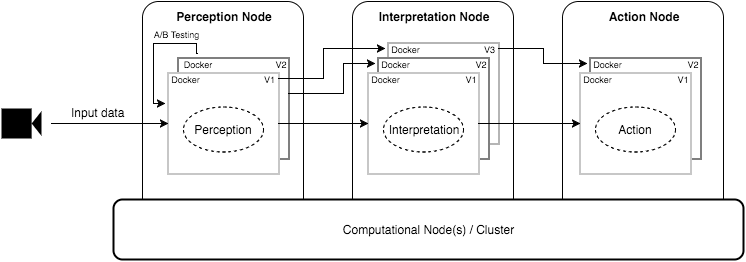
\includegraphics[width=1.0\textwidth]{./figure/containers.png}
      \caption{Run-time environment using Docker.}
       \label{containers}
\end{figure}


Figure \ref{containers} displays the utilization of docker in the context of a self-driving vehicle. The responsibilities are broken up into three computational nodes in which docker containers are running instances of the code separately. Further, the colored docker containers represents different versions of the separate nodes, where the interpretation node have three versions running separately. V1 in each node represent the latest working configuration while other versions are ran to test code which is under development. Aforementioned, this allows for safe and simple roll-backs as there will always be one working configuration as well as allowing for A/B testing between different containers. With an always working configuration, the development team can demonstrate the current status to stakeholders at any point in the development cycle. \\




\section{Problem Domain \& Motivation}
Our current society is increasingly depending upon real-time systems and automated solutions for many of the fundamental building blocks to the modern world. Such as systems used within financial, aviation, and automotive sectors. Sectors where these systems play an integral role in enabling automation to provide the services we all depend on today. With these industries advancing rapidly there is a need in understanding how software engineers and data scientists should best work while developing the systems that drives the progress. With work, we specifically imply the way the work flow of these software projects is structured in terms of integration- and deployment strategies.\\

There exists no evidence which presents argumentation regarding the impact state-of-art deployment strategies have on real-time systems. This creates a compelling gap in literature to explore this field by building argumentation which decision makers can rely upon when determining for which strategy is suitable for the application in question. The popularity of deployment strategies utilizing containers is steadily increasing, thus making it intriguing to understand the performance overhead introduced by containers such as Docker. While the implementation of virtualization technologies for deployment strategies brings many advantages, there still exists uncertainty to the disadvantage of how much, if any, performance overhead they carry.\\

It is of particular importance to understand this impact for decision makers responsible for determining deployment strategies for real-time systems. The rationale being that real-time systems are time constrained and must guarantee responses within a specified deadline. If the system is to violate the specified deadline it may lead to software failure, which can potentially be catastrophic in the context of autonomous self-driving vehicles. Therefore it is crucial to ensure that the execution environment and deployment context will allow the real-time application to stay within its specified time deadline. This is the gap in which the result of this research will seek to fulfil. By gaining knowledge of whether Docker carry extensive performance overhead which will rule it out from the list of possible approaches used for software deployment in real-time systems.\\

\section{Research Goal \& Research Questions}
This research seeks to understand the performance impact Docker have on real-time systems in the context of autonomous self-driving vehicles, as this context provides a solid connection to a real life case. By analysing data extracted from executions made in an application which is being implemented in vehicles today, we seek to find firm evidence which considers overhead introduced by code required for executing the real-time application (RQ1). Additional overhead may exist when executing the real-time application with other load bearing factors such as writing and reading to disk, reading from a camera feed. Thus making it important to understand how Docker affects the performance of the real-time application when including external components which are required in real life (RQ2).\\

\begin{enumerate}[label=\textbf{RQ\arabic*}]
	\item How does the respective execution environment influence the scheduling precision of the respective application?
	\item How does the respective execution environment influence the input/output performance of the respective application?\\
\end{enumerate}





Two sets of runs for each RQ where 1 is without load and 1 is with load. 
- we want to find wether there is a correlation between enviroment and performance depending on load

If something is not clear here, move that to section Background

\section{Contributions}

\section{Scope}
Contribution is only applicable in these conditions

\section{Structure of the article}


% information on:
	% RT Preempt Patch
	% OpenDaVINCI
	% Schedulers
	% Real Time Systems
	